\documentclass[11pt]{report}

%\usepackage{ucs}
\usepackage[latin1]{inputenc}
\usepackage[francais]{babel}
\usepackage[T1]{fontenc}
\usepackage{graphicx}
\usepackage{verbatim}
\usepackage{fancyhdr}
\usepackage{fancyvrb}
\usepackage{wrapfig}
\usepackage{pdfpages}
\usepackage{titlesec}
\usepackage{textcomp}
\usepackage{eurosym}
\usepackage{tikz}
\usepackage{colortbl}
%\usepackage[pdftex=true,
%           hyperindex=true,
%					 colorlinks=false]{hyperref}
%


\usepackage{vmargin}            % red�finir les marges
\setmarginsrb{1cm}{1cm}{1cm}{1cm}{1cm}{1cm}{1cm}{1.5cm}
% Marge gauche, haute, droite, basse- espace entre la marge et le texte �
% gauche, en  haut, � droite, en bas


%% Couleurs des �l�ments

\definecolor{logo}{rgb}{0.35,0.68,0.38}
\colorlet{section}{logo!80!black}
\colorlet{subsection}{logo}
\colorlet{subsubsection}{green!50!gray}
\colorlet{chapterfond}{logo}
\colorlet{titleboxcolor}{logo}
\colorlet{swot}{logo!30!white}

%\renewcommand{\bottomtitlespace}{15cm}%{.3\textheight}

\usepackage{messections}
\usepackage{redefinitionsdiverses}

\usepackage{subfig}

\begin{document}

\vfill


\includegraphics[height=2cm]{img/ferte} \hfill

\includegraphics[height=2cm]{img/PS} \hfill

\includegraphics[height=2cm]{img/eurobot} \\

\vfill

\hspace{-1.2em}\hrulefill
\begin{center}
	\Large{Coupe de France de Robotique 2011}\\
	\vspace{1cm}
	\textbf{\Huge{Chess'Up}}\\
\end{center}
\hrulefill

\hspace{1cm}
\begin{center}
\huge{�quipe Rob'Otter} \\
\vspace{.5cm}

\includegraphics[height=4cm]{img/beta}
\end{center}

\vfill


\includegraphics[height=1cm]{img/mdp} \hfill

\includegraphics[height=1cm]{img/altran} \hfill

\includegraphics[height=1cm]{img/rs} \\


\thispagestyle{empty}


\pagestyle{normal}

\begin{normalsize}

%%-----------------------------------------------------------------------------

\mychapter{Architecture �lectronique}


\begin{center}
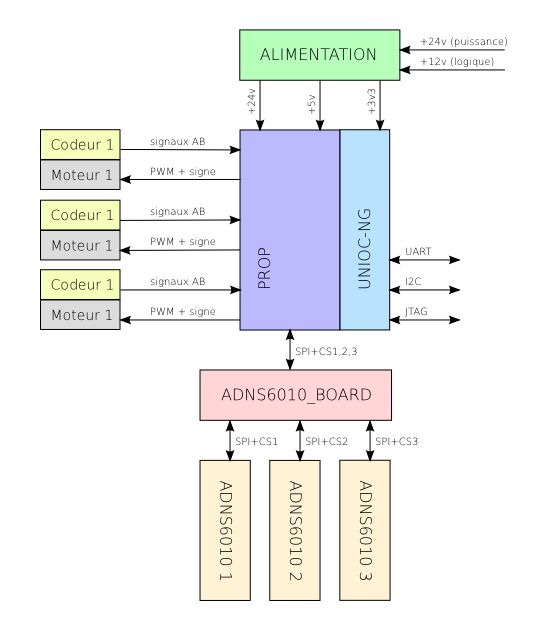
\includegraphics{imgs/archielec.png}
\end{center}




\mychapter{Asservissement}

\begin{center}
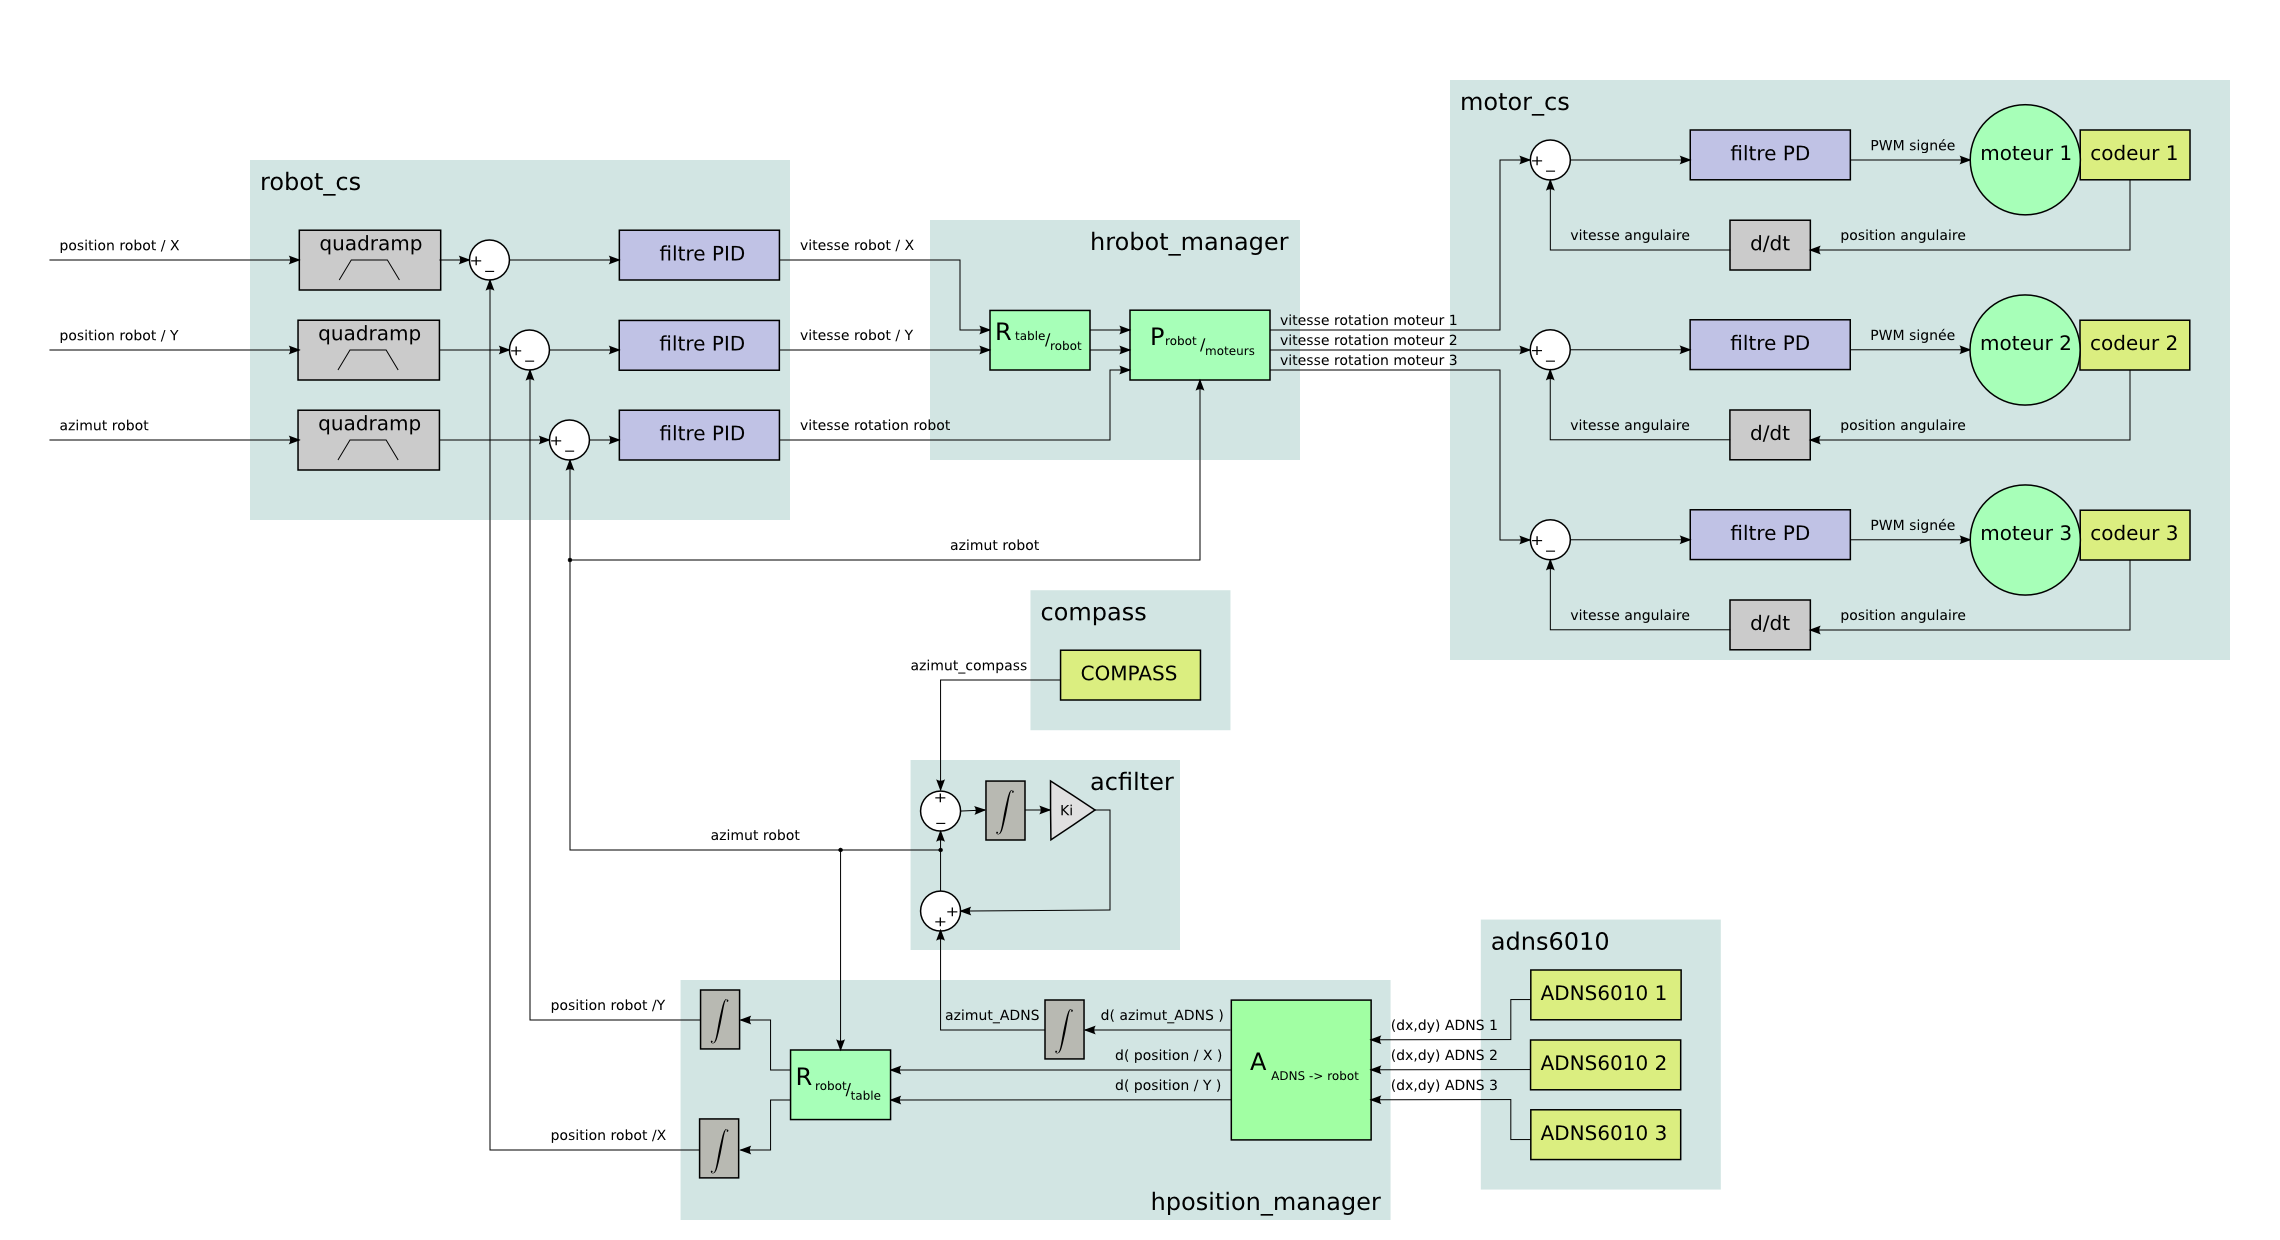
\includegraphics[width=1.0\textwidth]{imgs/asserv.png}
\end{center}


%%-------------------------------------------------------------------------------
\clearpage
\section{Asservissement en vitesse des moteurs}

\begin{center}
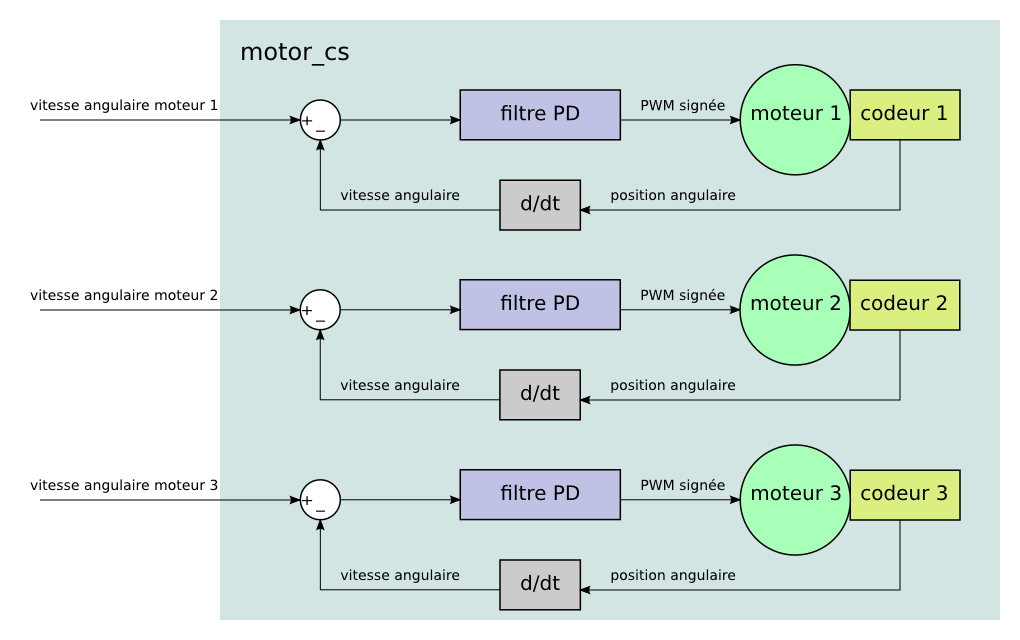
\includegraphics[width=0.8\textwidth]{imgs/motorcs.png}
\end{center}

Chaque moteur est individuellement asservi en vitesse par un r�gulateur PD
(Proportionnel,D�riv�e) et une codeur incr�mental HEDS5540 fix� � l'axe moteur.

\subsection{Consigne}
La consigne est ici une vitesse moteur exprim�e en \emph{pas
codeurs}/\emph{tick asservissement}.

\subsection{Correction}
La correction de l'asservissement est appliqu�e sous la forme d'une PWM + signe
envoy�e aux drivers moteurs, permettant de contr�ler le moteur en tension.

\subsection{Feedback}
L'information de vitesse est r�cup�r�e depuis les codeurs incr�mentaux HEDS5540,
branch�e sur le FPGA de l'UNIOC-NG, trait�s pour obtenir une position
absolue de l'axe moteur puis transmis � l'ATmega128 de l'UNIOC-NG.\\

Un filtre d�rivateur est appliqu�e sur la boucle de retour afin d'obtenir la
vitesse de rotation de l'axe moteur.

\clearpage
\subsection{Code}

L'asservissement en vitesse des moteurs est r�alis�  dans les fichiers
\verb$unioc_asserv/motor_cs.c$, \verb$unioc_asserv/motor_cs.h$ et 
\verb$unioc_asserv/motor_cs_config.h$.

\subsubsection{Initialisation}

\verb$unioc_asserv/main.c$ ligne 224 :\\
\begin{verbatim}
  //--------------------------------------------------------
  // Initialize control systems for motors
  printf("# Initializing motors control systems : ");
  motor_cs_init();
  printf("# OK\n");
\end{verbatim}

La fonction \verb$motor_cs_init$ assure l'initialisation des
\verb$control_system_managers$, filtres PID et PWM moteurs.

\subsubsection{Mise � jour}

La mise � jour de l'asservissement est effectu�e par la fonction
\verb$motor_cs_update()$ appell�e par la fonction \verb$hrobot_set_motors()$ 
du module \verb$hrobot_manager$ lors de l'envoi des consignes aux moteurs.

\verb$modules/devices/hrobot_manager/hrobot_manager.c$ ligne 74 :\\
\begin{verbatim}
  // set motors speeds
	if(hrs->motors_accessor)
		(hrs->motors_accessor)(hrs->motors_accessor_params, v0, v1, v2);
\end{verbatim}

Le pointeur \verb$hrs->motors_accessor$ est assign� � \verb$motor_cs_update()$ 
dans \verb$unioc_asserv/main.c$ ligne 208 :\\

\begin{verbatim}
  hrobot_set_motors_accessor(&system, motor_cs_update, NULL);
\end{verbatim}

%%-------------------------------------------------------------------------------

\clearpage

\section{Propulsion vectorielle}

\begin{center}
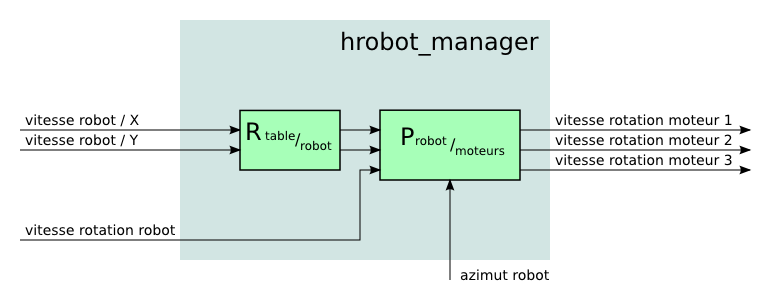
\includegraphics[width=0.6\textwidth]{imgs/hrobot.png}
\end{center}

\subsection{Th�orie}

La propulsion vectorielle permet de transformer une consigne en vitesse exprim�e
dans le rep�re li� au robot $R_{robot}$ :
\begin{equation}
\left(\begin{array}{c} v_x\\v_y\\\omega_z\end{array}\right)_{R_{robot}}
\end{equation}

En une consigne en vitesse sur chaque moteur :
\begin{equation}
\left(\begin{array}{c}v_{M_1}\\v_{M_2}\\v_{M_3}\end{array}\right)_{R_{moteurs}}
\end{equation}

\begin{center}
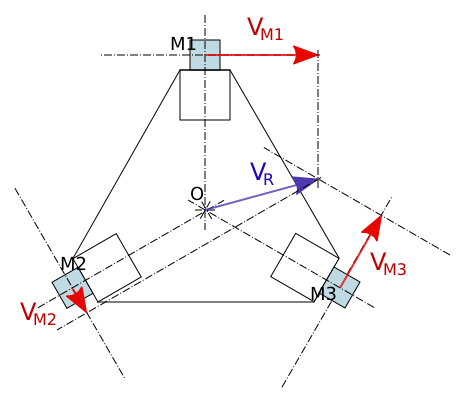
\includegraphics[width=0.5\textwidth]{imgs/prop_vect.png}
\end{center}

Soit $\overrightarrow{u_{M_1}}$, $\overrightarrow{u_{M_2}}$,
$\overrightarrow{u_{M_3}}$ respectivement les vecteurs unitaires
colin�aires au diam�tre de chaque roue et appartenant au plan
$(\vec{x},\vec{y})$, chaque vecteur positif dans le sens de pouss�e positive
de chaque moteur.\\
Soit $R$ la distance entre le point d'appui d'une omniwheel et le centre du
robot.\\
On  pose $\overrightarrow{V_{robot/table}}_O =
\left(\begin{array}{c}v_x\\v_y\\0\end{array}\right)_O$
vecteur vitesse du robot en $O$ dans le rep�re li� � la table.\\

\vskip 1cm

On effectue le d�placement du torseur cin�matique du robot en $O$
aux points de contacts de chaque roue $M_1$, $M_2$ et $M_3$.\\

Au point $O$ le torseur cin�matique du robot est :
\begin{equation}
\left\{ \nu_{robot/table} \right\}
%%
= \left\{ \begin{array}{c}
\omega.\overrightarrow{z} % w.z
\\
\overrightarrow{V_{robot/table}}_O
\end{array} \right\}_{O}
%%
= \left\{ \begin{array}{cc}
v_x & 0\\
v_y & 0\\
0 & \omega_z\\
\end{array} \right\}_{O}
%%
\end{equation}

D�placement du torseur en $M_1$ :
\begin{eqnarray}
\left\{ \nu_{robot/table} \right\} &
%%
= & \left\{ \begin{array}{c}
\omega_z.\overrightarrow{z} % w.z
\\
\overrightarrow{V_{robot/table}}_O
\end{array} \right\}_{O} \\
%%
& = & \left\{ \begin{array}{c}
\omega_z.\overrightarrow{z} % w.z
\\
\overrightarrow{V_{robot/table}}_O + \overrightarrow{OM_1} \wedge
\omega_z.\overrightarrow{z}
\end{array} \right\}_{M_1}\\
%%
& = & \left\{ \begin{array}{c}
\omega_z.\overrightarrow{z} % w.z
\\
\overrightarrow{V_{robot/table}}_O + R.\omega_z.\overrightarrow{u_{M_1}}
\end{array}\right\}_{M_1}
\end{eqnarray}

On obtient de m�me en $M_2$ et $M_3$ :
\begin{equation}
\left\{ \nu_{robot/table} \right\} 
=
\left\{ \begin{array}{c}
\omega_z.\overrightarrow{z} % w.z
\\
\overrightarrow{V_{robot/table}}_O + R.\omega_z.\overrightarrow{u_{M_2}}
\end{array}\right\}_{M_2}
\end{equation}

\begin{equation}
\left\{ \nu_{robot/table} \right\} 
=
\left\{ \begin{array}{c}
\omega_z.\overrightarrow{z} % w.z
\\
\overrightarrow{V_{robot/table}}_O + R.\omega_z.\overrightarrow{u_{M_3}}
\end{array}\right\}_{M_3}
\end{equation}

Chaque omniwheel $n$ ne peut fixer la vitesse que suivant l'axe
$\overrightarrow{u_{M_n}}$, on obtient donc, en notant $\theta_{M_n}$ 
l'orientation respective de chaque vecteur $u_{Mn}$ :
\begin{eqnarray}
v_{M_n} & = & \overrightarrow{V_{robot/table}}_{M_n} .
\overrightarrow{u_{M_n}}\\
%%
        & = & ( \overrightarrow{V_{robot/table}}_O +
R.\omega_z.\overrightarrow{u_{M_n}} ).\overrightarrow{u_{M_n}}\\
%%
        & = & \left(\begin{array}{c}v_x\\v_y\\0\end{array}\right).
\left(\begin{array}{c}\cos \theta_{M_n}\\\sin \theta_{M_n}\\0\end{array}\right)
+ R.\omega_z\\
%%
        & = & v_x.\cos \theta_{M_n} + v_y.\sin \theta_{M_n} + R.\omega_z
\end{eqnarray}

Ce qui donne le syst�me d'�quations suivant :
\begin{eqnarray}
v_{M_1} = v_x.\cos \theta_{M_1} + v_y.\sin \theta_{M_1} + R.\omega_z\\
v_{M_2} = v_x.\cos \theta_{M_2} + v_y.\sin \theta_{M_2} + R.\omega_z\\
v_{M_3} = v_x.\cos \theta_{M_3} + v_y.\sin \theta_{M_3} + R.\omega_z
\end{eqnarray}

\subsection{Code}

\subsubsection{Initialisation}

Le module \verb$hrobot_manager$ est initialis� dans le fichier \verb$main.c$
lignes 205 � 211 :
\begin{verbatim}
  printf("# Initializing robot manager : ");
  hrobot_init(&system);
  hrobot_set_motors_accessor(&system, motor_cs_update, NULL);
  printf("# OK\n");

  printf("# Robot manager is GO\n\n");
\end{verbatim}

\subsubsection{Mise � jour}

Ces transformations sont impl�ment�es dans la fonction \verb$hrobot_set_motors$ 
du module \verb$hrobot_manager$ aux lignes 62 � 70 :
\begin{verbatim}
  // project speed vector on each motor
  v0 = vx*HROBOT_MOTOR0_COS_COURSE + vy*HROBOT_MOTOR0_SIN_COURSE;
  v1 = vx*HROBOT_MOTOR1_COS_COURSE + vy*HROBOT_MOTOR1_SIN_COURSE;
  v2 = vx*HROBOT_MOTOR2_COS_COURSE + vy*HROBOT_MOTOR2_SIN_COURSE;
  
  // 
  v0 += omega;
  v1 += omega;
  v2 += omega;
\end{verbatim}

Notons que dans la version pr�sent�e du code aucun effort de mise en conformit�
des unit�s n'a �t� effectu�e $R$ �tant �gal � $1$ ici.



%%-------------------------------------------------------------------------------

\section{Positionnement}


\begin{center}
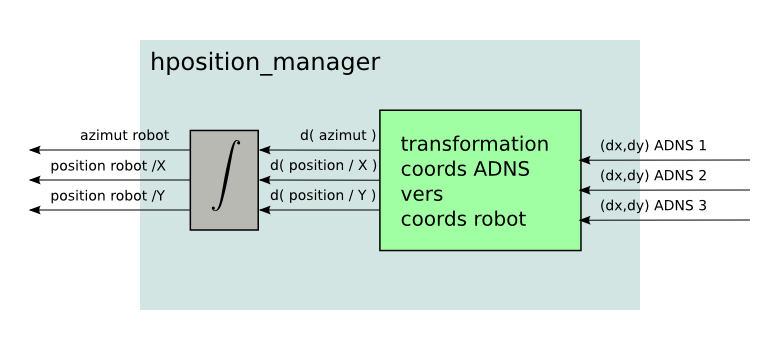
\includegraphics[width=0.7\textwidth]{imgs/hposition.png}
\end{center}


\subsection{Transformation vitesses ADNS vers vitesses robot}

\subsubsection{Th�orie}

La carte ADNS6010 donne les vitesses de d�placement de chaque capteur dans son
rep�re.

\begin{center}
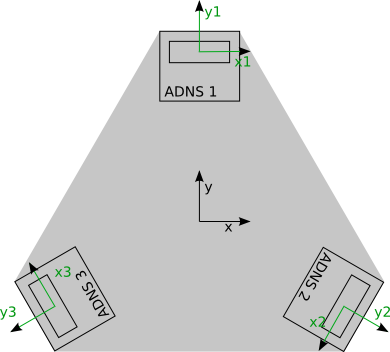
\includegraphics[width=0.5\textwidth]{imgs/adns6010.png}
\end{center}

Soit le vecteur $\left(\begin{array}{c}
v_{x1}\\v_{y1}\\v_{x2}\\v_{y2}\\v_{x3}\\v_{y3}\end{array}\right)$
repr�sentant les informations de vitesses renvoy�es par le capteur ADNS.\\

Sachant que chaque rep�re ADNS est une transformation lin�aire du rep�re du robot on
peut dire, en notant $\left(\begin{array}{c} 
v_x\\v_y\\\omega_z\end{array}\right)_{R_{robot}}$ la vitesse du robot, qu'il existe une matrice $A$
telle que :\\

\begin{equation}
\left(\begin{array}{c} 
v_x\\v_y\\\omega_z\end{array}\right)_{R_{robot}}
=A
\left(\begin{array}{c}
v_{x1}\\v_{y1}\\v_{x2}\\v_{y2}\\v_{x3}\\v_{y3}\end{array}\right)
\end{equation}

La matrice $A$ est donc une matrice 3x6 obtenue par identification du capteur
ADNS.
\begin{equation}
A = \left(\begin{array}{cccccc}
a_{00}& a_{01}& a_{02}& a_{03}& a_{04}& a_{05}\\
a_{10}& a_{11}& a_{12}& a_{13}& a_{14}& a_{15}\\
a_{20}& a_{21}& a_{22}& a_{23}& a_{24}& a_{25}\\
\end{array}
\right)
\end{equation}

\subsubsection{Code}

\paragraph{Initialisation}

Le module \verb$hposition_manager$ est initialis� dans le fichier \verb$main.c$
lignes 216 � 221 :
\begin{verbatim}
  printf("# Initializing position manager : ");
  hposition_init( &position );
  hposition_set( &position, 0.0, 0.0, 0.0 );
  printf("# OK\n");

  printf("# Position manager is GO\n\n");
\end{verbatim}

\paragraph{Mise � jour}

La transformation, r�duite � un produit matriciel, est impl�ment� dans la 
fonction \verb$hposition_update$ du module \verb$hposition_manager$ aux lignes
119 � 137.

\begin{verbatim}
  //----------------------------------------------------------
  // Transform speed in ADNS coordinates to robot coordinates

  // compute speed in ADNS coordinates
  for(i=0;i<6;i++)
    v[i] = hpos->pAdnsVectors[i] - adns6010.vectors[i];

  // update previous ADNS vectors
  for(i=0;i<6;i++)
    hpos->pAdnsVectors[i] = adns6010.vectors[i];

  // for each robot coordinate (x,y,a) compute a dx of mouvement
  for(k=0;k<3;k++)
  {
    dp[k] = 0.0;
    
    // for each ADNS coordinate (vx1,vy1,vx2,vy2,vx3,vy3) 
    for(i=0;i<6;i++)
    {
      dp[k] += hrobot_adnsMatrix[k][i]*v[i];
    }
  }
\end{verbatim}

\subsection{Int�gration des vitesses ADNS}

\subsubsection{Th�orie}

L'�l�ment
$\left(\begin{array}{c}v_x\\v_y\\\omega_z\end{array}\right)_{R_{robot}}$ calcul�
pr�c�dement est donn� dans le rep�re li� au capteur ADNS donc � $R_{robot}$
rep�re li� au robot.\\

Il convient donc de le transformer par une rotation de $\alpha$, angle du robot
par rapport � la table.

\subsubsection{Code}

L'int�gration de l'�l�ment de position calcul� est effectu� � la suite dans la
fonction \verb$hposition_update$ aux lignes 142 � 147.

\begin{verbatim}
  alpha = hpos->position.alpha;

  x = hpos->position.x + dp[HROBOT_DX]*cos(alpha) - dp[HROBOT_DY]*sin(alpha);
  y = hpos->position.y + dp[HROBOT_DX]*sin(alpha) + dp[HROBOT_DY]*cos(alpha);

  alpha += dp[HROBOT_DA];
\end{verbatim}


\section{Asservisement en position}

\begin{center}
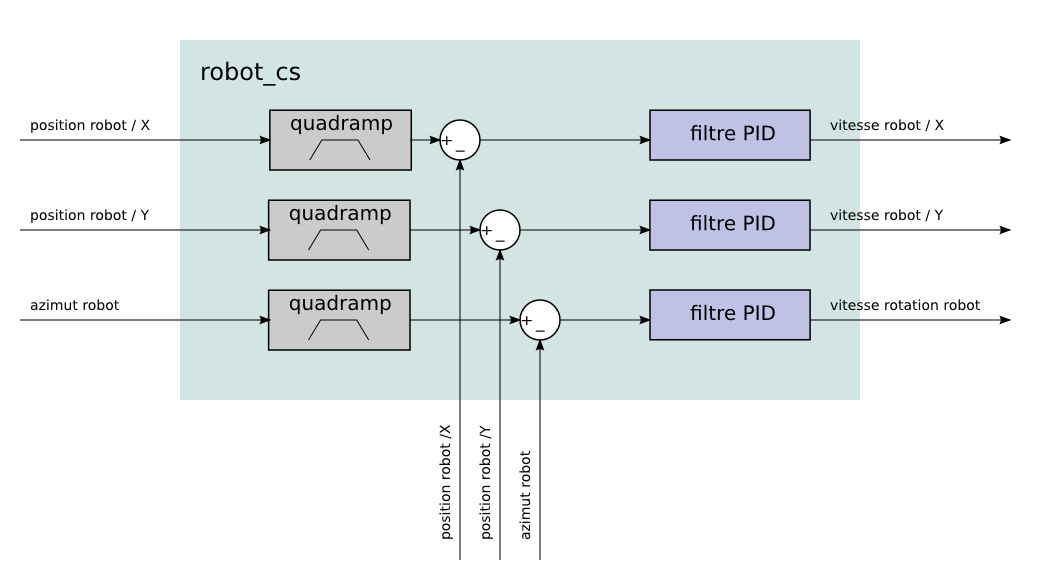
\includegraphics[width=0.8\textwidth]{imgs/robot_cs.png}
\end{center}

Le robot est asservi en position par un r�gulateur PID sur chaque dimension : 
translation suivant $\vec{x}$, translation suivant $\vec{y}$, rotation suivant
$\vec{z}$.
La derni�re �tape consiste en une rotation du vecteur afin de le passer du
rep�re $R_{table}$ au rep�re $R_{robot}$.

\subsection{Boucles d'asservissement}

\subsubsection{Consigne}
La consigne est une position exprim�e en mm et en radians.\\

Un filtre \emph{quadramp} est appliqu� � la consigne permettant de limiter ses
d�riv�es premi�res et secondes, limitant ainsi l'acc�l�ration et la vitesse du
robot.

\subsubsection{Correction}
La correction de l'asservissement est un vecteur vitesse pass� en consigne
� l'asservissement des moteurs.

\subsubsection{Feedback}
L'information de position est r�cup�r�e depuis le module
\verb$hposition_manager$, calcul�e depuis le retour de la carte ADNS6010.

\subsubsection{Code}

L'asservissement en position du robot est r�alis� dans les fichiers
\verb$unioc_asserv/robot_cs.c$ et \verb$unioc_asserv/robot_cs.h$.

\subsubsection{Initialisation}

\verb$unioc_asserv/main.c$ ligne 230 :\\
\begin{verbatim}
  // Initialize control systems for robot
  printf("# Initializing robot control systems : ");
  robot_cs_init(&robot_cs);
  robot_cs_set_hrobot_manager(&robot_cs,&system);
  robot_cs_set_hposition_manager(&robot_cs,&position);
  printf("# OK\n");
\end{verbatim}

La fonction \verb$robot_cs_init$ assure l'initialisation des
\verb$control_system_managers$, filtres PID et quadramps.

\subsubsection{Mise � jour}

La mise � jour de l'asservissement est effectu�e par la fonction
\verb$robot_cs_update()$ appell�e sur interruption par le module
\verb$scheduler$ :

\verb$unioc_asserv/main.c$ ligne 324 :\\
\begin{verbatim}
 // Unleash control systems
  scheduler_add_periodical_event_priority(&robot_cs_update, &robot_cs,
                                            10,100);
\end{verbatim}

\subsection{Changement de rep�re}

\subsubsection{Th�orie}

La correction calcul�e par l'asservissement en position est exprim�e dans le
rep�re li� � la table de jeu $R_{table}$.\\
Avant de l'envoyer aux asservissements moteurs il faut effecteur un changement
de rep�re de $R_{table}$ vers $R_{robot}$.\\

\begin{center}
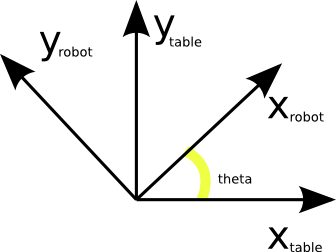
\includegraphics[width=0.25\textwidth]{imgs/rep.png}
\end{center}

On a :

\begin{equation}
\left(\begin{array}{c}
v_x\\v_y\\\omega_z
\end{array}
\right)_{R_{table}}
=
\left(\begin{array}{ccc}
\cos(\theta)&-\sin(\theta)&0\\
\sin(\theta)&\cos(\theta)&0\\
0&0&1\\
\end{array}
\right)
\left(\begin{array}{c}
v_x\\v_y\\\omega_z
\end{array}
\right)_{R_{robot}}
\end{equation}

\begin{equation}
\left(\begin{array}{c}
v_x\\v_y\\\omega_z
\end{array}
\right)_{R_{robot}}
=
\left(\begin{array}{ccc}
\cos(\theta)&\sin(\theta)&0\\
-\sin(\theta)&\cos(\theta)&0\\
0&0&1\\
\end{array}
\right)
\left(\begin{array}{c}
v_x\\v_y\\\omega_z
\end{array}
\right)_{R_{table}}
\end{equation}

\subsubsection{Code}

Le changement de rep�re est effectu� dans la fonction \verb$robot_cs_update()$
:\\
\begin{verbatim}
  vx_t     = cs_get_out(&csm_x);
  vy_t     = cs_get_out(&csm_y);
  omegaz_t = cs_get_out(&csm_angle);

  hposition_get(rcs->hpm, &hvec);

  alpha = -hvec.alpha;
 
  vx_r = vx_t*cos(alpha) - vy_t*sin(alpha);
  vy_r = vx_t*sin(alpha) + vy_t*cos(alpha);
\end{verbatim}

\section{Fonctionnement nominal}

\subsection{Initialisation}

La fonction \verb$hposition_update$ assurant la mise � jour de la position du
robot � partir des informations retourn�es par les ADNS est appell�e sur
interruption, par le biais du module scheduler.\\
L'appel est initialis� dans \verb$main.c$ :\\
\begin{verbatim}
scheduler_add_periodical_event_priority(&hposition_update, &position, 400, 50);
\end{verbatim}

\vskip 0.5cm

La fonction \verb$robot_cs_update$ assurant la mise � jour de l'asservissement
est appell�e elle aussi sur interuption, l'appel est initialis� dans
\verb$main.c$ :\\
\begin{verbatim}
scheduler_add_periodical_event_priority(&robot_cs_update, &robot_cs, 10, 100);
\end{verbatim}


\subsection{Mise � jour de l'asservissement}

La mise � jour de l'asservissement se d�roule de la mani�re suivante :
\begin{itemize}
\item appel de \verb$robot_cs_update$, mise � jour des asservissements en
translation suivant $\vec{x}$, translation suivant $\vec{y}$ et angle selon
$\vec{z}$;
\item appel de \verb$hrobot_set_motors$ avec les valeurs calcul�es par les 3
asservissements en position, afin de transformer une consigne en vitesse dans le
rep�re du robot vers une consigne en vitesse sur chaque moteur;
\item appel de \verb$motor_cs_update$  avec les consignes en vitesse de chaque
moteur, mise � jour des asservissement en vitesses des 3 moteurs;
\item mise � jour des PWMs avec les valeurs calcul�es par les asservissements en
vitesse.
\end{itemize}


%%-----------------------------------------------------------------------------

\mychapter{Identification du capteur ADNS}

\section{Th�orie}

Le capteur de position constitu� de 3 capteurs optiques ADNS6010 n'est pas
parfaitement ajust� dans les axes de la base roulante et il est, par cons�quent,
difficile de calculer la matrice $A$ vue pr�c�dement a partir des mesures du
capteur.

\begin{equation}
\left(\begin{array}{c} 
v_x\\v_y\\\omega_z\end{array}\right)
=A
\left(\begin{array}{c}
v_{x1}\\v_{y1}\\v_{x2}\\v_{y2}\\v_{x3}\\v_{y3}\end{array}\right)
\end{equation}


La m�thode est donc d'effectuer une s�rie de mesure de couples $(U,V)$ o� 
$U = \left(\begin{array}{c}v_x\\v_y\\\omega_z\end{array}\right)$ et
$V = \left(\begin{array}{c}v_{x1}\\v_{y1}\\v_{x2}\\v_{y2}\\v_{x3}\\
v_{y3}\end{array}\right)$.\\

Par exemple effectuer depuis le point
$\left(\begin{array}{c}0\\0\\0\end{array}\right)$ 
une translation de $400 mm$ suivant l'axe $\vec{x}$ donne 
le couple $(U_0,V_0)$ suivant :

\begin{equation}
\left(
\left(\begin{array}{c}400\\0\\0\end{array}\right)
,
\left(\begin{array}{c}30110\\-17327\\-30676\\-17198\\972\\35188
\end{array}\right)
\right)
\end{equation}

Il reste � effectuer un grand nombre de mesure sur des
coordonn�es vari�es et d'ensuite identifier la matrice $A$ au moyen d'un
algorithme d'identification.

\section{Code}

L'identification est effectu�e au moyen de la m�thode ARMA sous SciLab
gr�ce au script\\\verb$unioc_asserv/scilab/adns_calibration.sci$.



\end{normalsize}
\end{document}
